\documentclass{article}
\usepackage{fontspec}
\usepackage{polyglossia}
\setdefaultlanguage{french}
\usepackage[a4paper,margin=1cm]{geometry}

\usepackage{amsmath}
\usepackage{array}
\usepackage{auto-pst-pdf}
\usepackage{booktabs}
\usepackage{cite}
\usepackage{graphicx}
\usepackage{lmodern}
\usepackage{marvosym}
\usepackage{mathrsfs}
\usepackage{minted}
\usepackage{multicol}
\usepackage{multirow}
\usepackage{paralist}
\usepackage{schemabloc}
\usepackage{siunitx}
\usepackage{soul}
\usepackage{tikz}
\usepackage[european,cuteinductors,siunitx]{circuitikz}
\usepackage{url,hyperref}
\usepackage{verbatim}
\usepackage{xunicode,xltxtra}

\title{
\includegraphics{../../../images/inp-enseeiht} \\ ~ \\ ~ \\ ~ \\ ~ \\ TP n°2 \\ Placement et routage d’un FPGA}
\author{Guilhem Saurel}
\date{\oldstylenums{\today}}

\begin{document}

\begin{titlepage}
    \setcounter{page}{0}
    \maketitle
    \thispagestyle{empty}
\tableofcontents
\end{titlepage}


\section{Compteur synchrone}
\subsection{Bloc F}
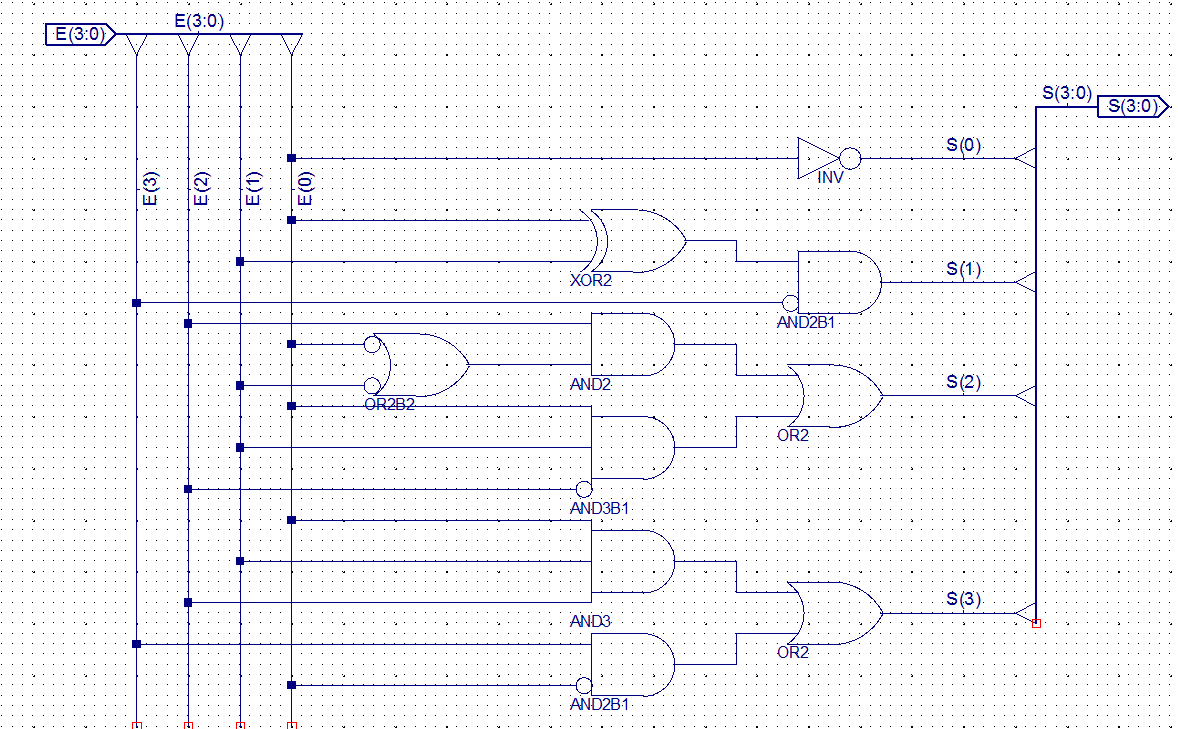
\includegraphics[width=\linewidth]{bloc_combinatoire}
\subsection{Compteur}
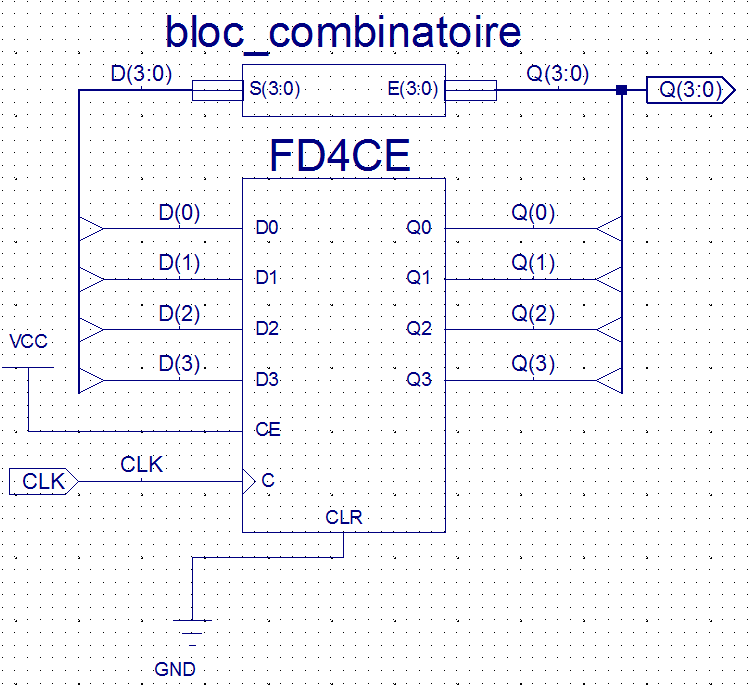
\includegraphics[width=\linewidth]{compteur_decade}

\section{Testbench \& Simulation}
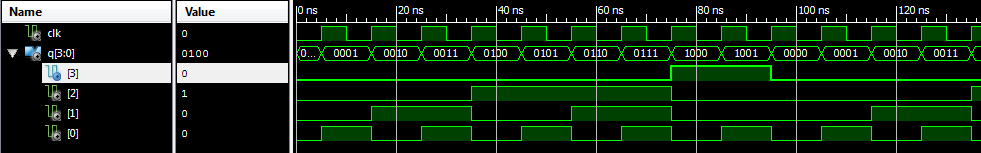
\includegraphics[width=\linewidth]{Testbench}
Nous pouvons voir que ce compteur compte.

\section{FPGA Editor}
\subsection{Blocks}
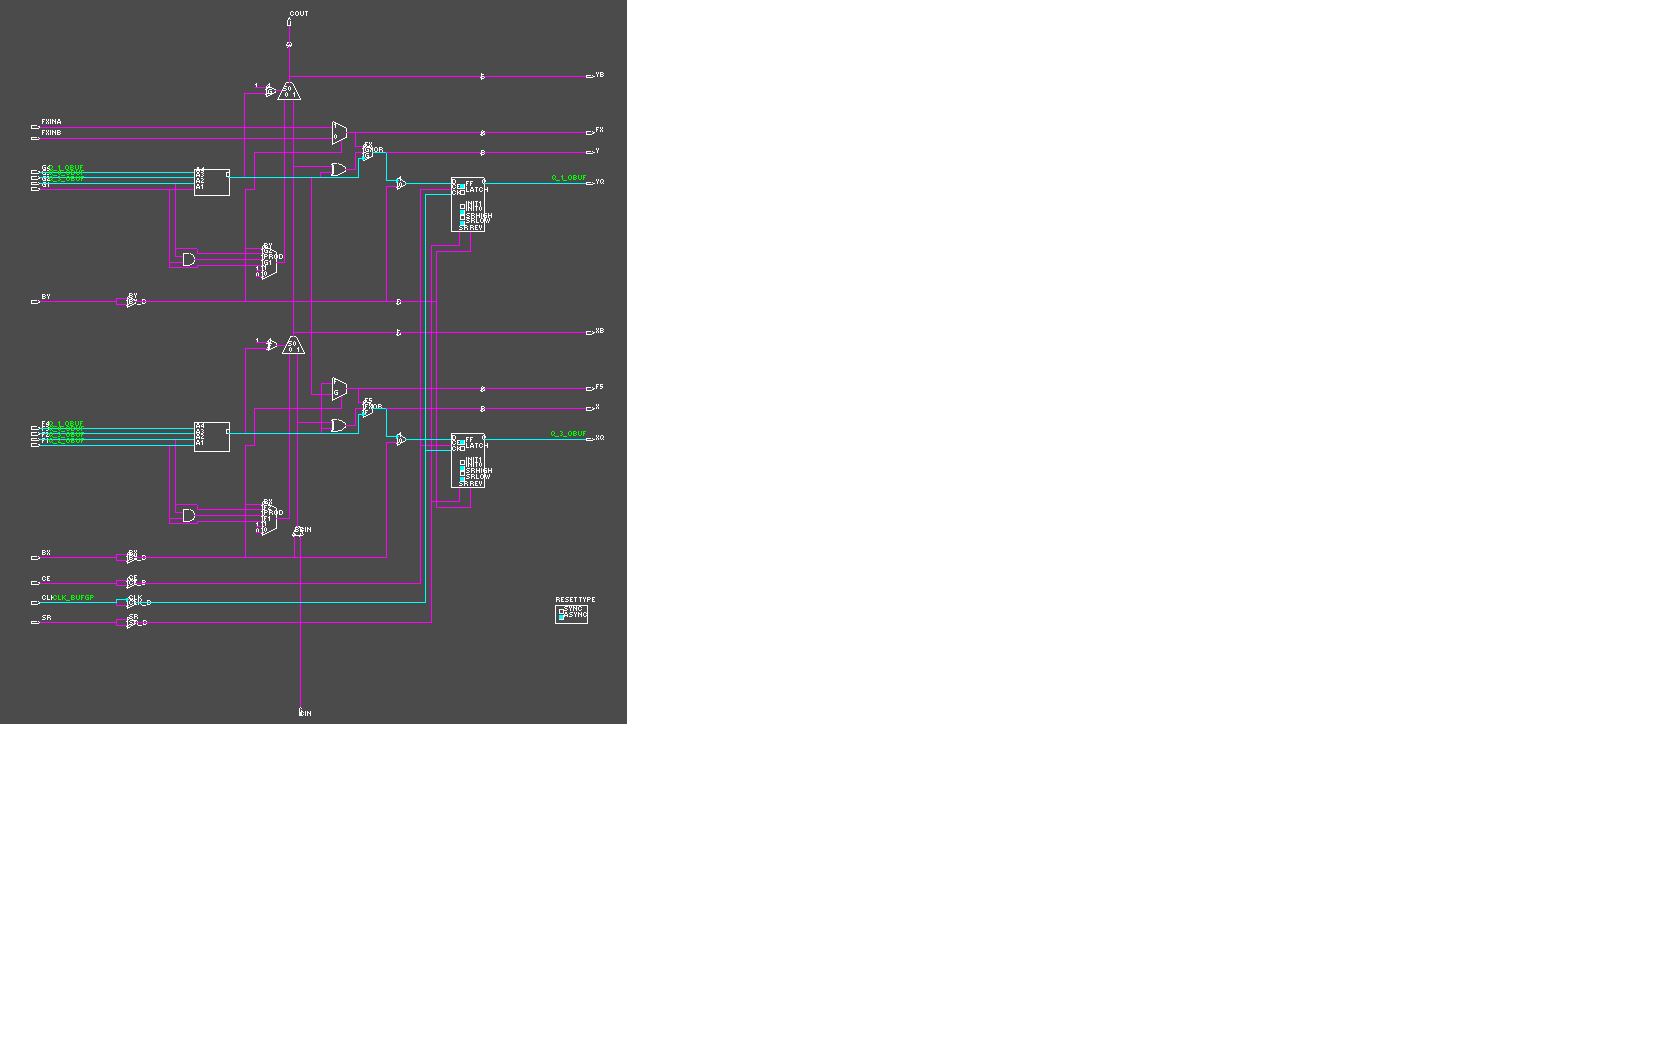
\includegraphics{block1}
On vérifie bien que les fonctions logiques dans les LUT sont celles que l’on attendait.

Par exemple, pour \verb|Q(2)|, on a bien \verb|<G>=((~A4*(A3*A1))+(A4*(~A3+~A1)));|, où
\verb|A1| correspond à \verb|Q(0)|, \verb|A3| à \verb|Q(1)| et \verb|A4| à \verb|Q(2)|.

\subsection{delays}
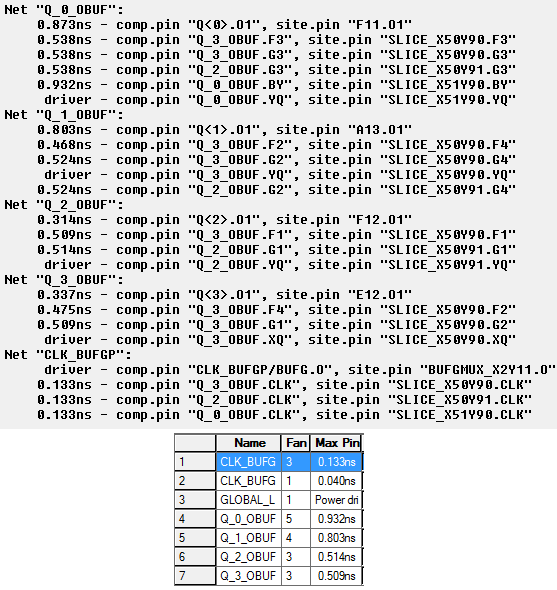
\includegraphics{delay}

On observe que le temps le plus long est de \verb|0.932ns|, entre la bascule 0 et elle-même.
C’est donc la connexion «la plus critique».

pour les temps de propagation de l’horloge, on remarque que le signal arrive en même temps partout.
C’est dû à la technologie utilisé pour ce signal spécifique.

\section{temps de propagation}
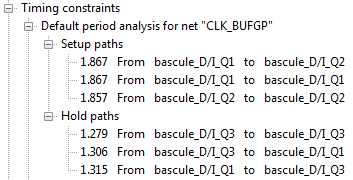
\includegraphics{temps_de_propagation}

Ici, le temps de propagation maximal est de 1.867ns, donc, en arrondissant, ça nous donne une
fréquence de fonctionnement maximale de 500MHz.

\section{Plan Ahead}
\subsection{Placement automatique}

En placement initial, on remarque que les composants sont placés proches les uns des autres:

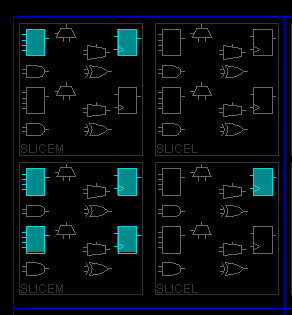
\includegraphics{plan_ahead}.

\subsection{Placement manuel}

Pour observer l’effet de ce positionnement sur les temps de propagation, on «casse» ce placemente:

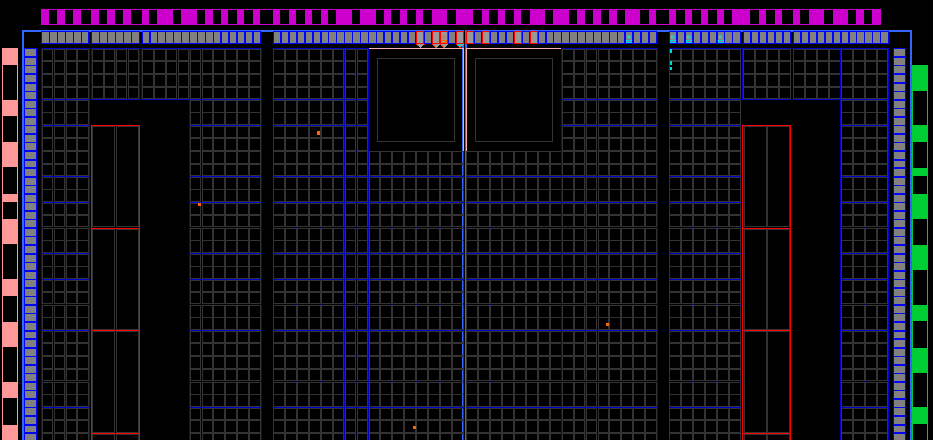
\includegraphics[width=\linewidth]{plan_ahead_casse}

Ce qui se répercute dans le fichier ucf:

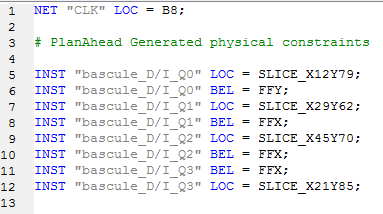
\includegraphics{plan_ahead_casse_ucf}

On observe logiquement des temps de propagation plus importants:

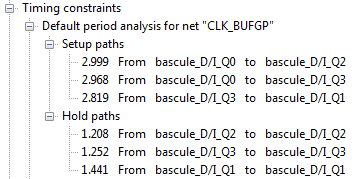
\includegraphics{temps_de_propagation_casse}

La fréquence maximale de fonctionnement devient alors approximativement de 333MHz.

\subsection{Placement semi-automatique}

Cette fois-ci, on délimite une zone dans le centre du FPGA:

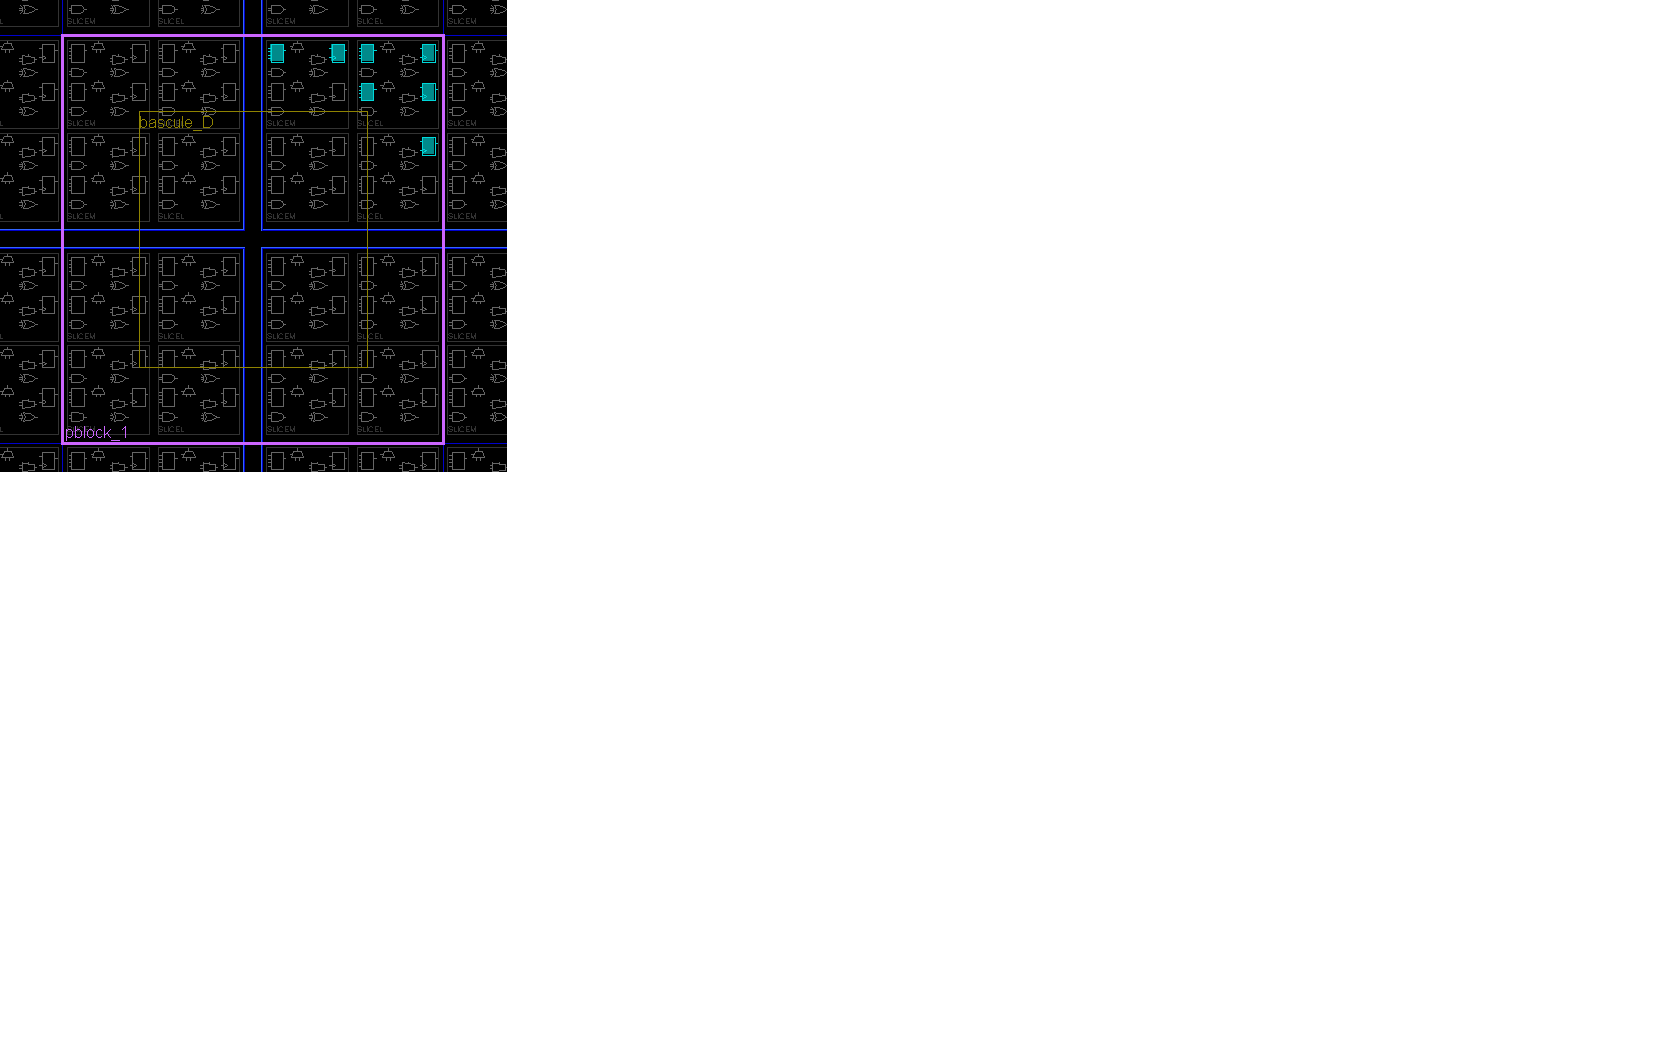
\includegraphics{plan_ahead_zone}

Ce qui agit à nouveau sur le fichier de contrainte:

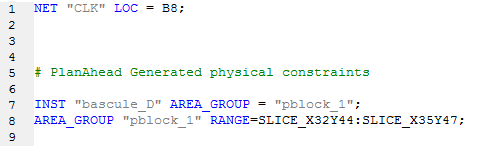
\includegraphics{plan_ahead_zone_ucf}

Et les temps de propagation sont revenus à un niveau normal:

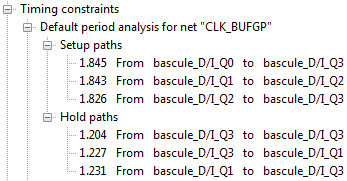
\includegraphics{temps_de_propagation_zone}


\section{Contraintes temporelles sur l’horloge}

Si l’on ajoute un contrainte temporelle de période de 2ns, tout se passe bien:

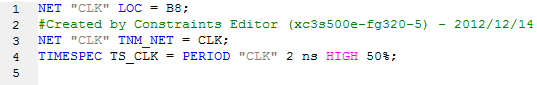
\includegraphics{time_constraint_ucf}

Par contre, si on réduit cette période à 1ns, ce qui est censé être trop rapide par rapport à nos temps de propagation,
ISE va nous avertir du problème:

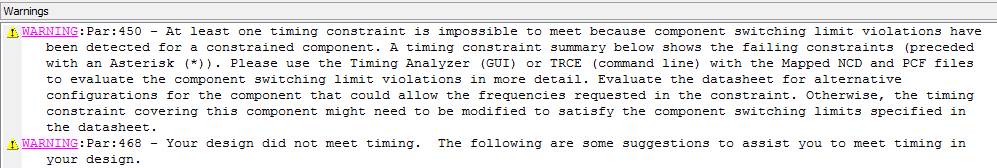
\includegraphics[width=\linewidth]{time_constraint_warning_1ns}

Et Plan Ahead va également indiquer l’erreur:

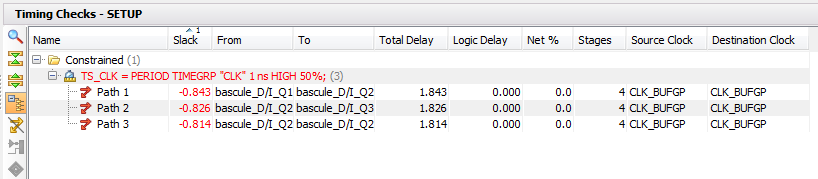
\includegraphics[width=\linewidth]{time_constraint_warning_1ns_plan_ahead}

\section{Simulation post-routage}

En regardant la clock des bascules D et les signaux, on voit que c’est la bascule correspondant au signal Q1 qui est la plus
longue, et elle présente une latence de 1.666 ns:

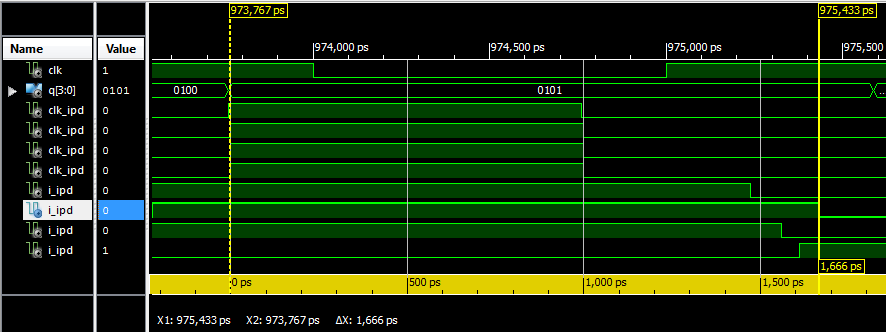
\includegraphics{entree_bascule}

\section{Implémentation dans le FPGA}

\subsection{Vérification du compteur}

Notre compteur continue de compter:

\includegraphics[width=\linewidth]{compteur}

\subsection{Délais}

La résolution de l’oscilloscope ne nous permet pas d’avoir des mesures de l’ordre de la ps, mais on voit quand
même quels signaux sont en avance:

\includegraphics[width=\linewidth]{temps_propagation}


\end{document}

